\makeatletter
\def\input@path{{../styles/}{../../styles/}{../../../styles/}{../}{../../}{../../../}}
\makeatother
\documentclass{ee102_notes}
% macros.tex - Course meta information
\renewcommand{\course}{EE 102}
\renewcommand{\coursetitle}{Signal Processing and Linear Systems}
\renewcommand{\instructor}{Ayush Pandey}
\renewcommand{\semester}{Fall}
\renewcommand{\year}{2025}
\renewcommand{\shorttitle}{Week 1: Introduction to Signals}
% Use \renewcommand to avoid 'already defined' errors

% The following packages can be found on http:\\www.ctan.org
% \usepackage{graphics} % for pdf, bitmapped graphics files
%\usepackage{epsfig} % for postscript graphics files
%\usepackage{mathptmx} % assumes new font selection scheme installed
%\usepackage{times} % assumes new font selection scheme installed
\usepackage{amsmath} % assumes amsmath package installed
\usepackage{amssymb,mathtools}  % assumes amsmath package installed
\usepackage{xcolor}
\usepackage{pgfplots,subcaption}
\usepackage[hidelinks]{hyperref}
\usepackage{verbatim}
\usepackage{graphicx}
\usepackage{listings}
\usepackage{fancyhdr}
% \usepackage{geometry}
\usepackage{siunitx}
\usepackage[most]{tcolorbox}
\usepackage{enumitem}
\usepackage{environ}
% -------- listings (Python) ----------
\lstdefinestyle{py}{
  language=Python,
  basicstyle=\ttfamily\small,
  keywordstyle=\color{blue!60!black}\bfseries,
  commentstyle=\color{green!40!black},
  stringstyle=\color{orange!60!black},
  showstringspaces=false,
  columns=fullflexible,
  frame=single,
  framerule=0.3pt,
  numbers=left,
  numberstyle=\tiny,
  xleftmargin=1em,
  tabsize=2,
  breaklines=true,
}

\usepackage[american]{circuitikz}
\usepackage{tikz}
\usetikzlibrary{arrows.meta,positioning,calc,angles,quotes}
\tikzset{
  >={Latex[length=2.2mm]},
  block/.style={draw, thick, rectangle, minimum height=10mm, minimum width=24mm, align=center},
  gain/.style={block, minimum width=14mm},
  sum/.style={draw, thick, circle, inner sep=0pt, minimum size=6mm},
  conn/.style={-Latex, thick},
}
\usepackage{caption}    
\usepackage{lscape}
\usepackage{soul}
\usepackage{physics}
\usepackage{hyperref}
\hypersetup{
    colorlinks=true,
    linkcolor=blue,
    filecolor=magenta,      
    urlcolor=blue,
    pdftitle={week1_notes},
    pdfpagemode=FullScreen,
}
%\usepackage{float} 

%\usepackage[demo]{graphicx}
\pgfplotsset{compat=1.18}
% \usepgfplotslibrary{fillbetween}

\newsavebox{\measurebox}

\let\proof\relax\let\endproof\relax


\def\abs#1{\left\lvert#1\right\rvert}
\let\proof\relax
\let\endproof\relax
\usepackage{amsthm}
\usepackage{accents}
\usepackage{relsize}
\newcommand{\ubar}[1]{\underaccent{\bar}{#1}}
\newtheorem{theorem}{Theorem}
\newtheorem{corollary}{Corollary}[theorem]
\newtheorem{lemma}{Lemma}
\newtheorem{proposition}{Proposition}
\newtheorem{statement}{Statement}

\theoremstyle{definition}
\newtheorem{definition}{Definition}
 
\theoremstyle{remark}
\newtheorem*{remark}{Remark}
\theoremstyle{remark}
\newtheorem*{claim}{Claim}
\setlength{\parindent}{0cm}
\newenvironment{nalign}{
    \begin{equation}
    \begin{aligned}
}{
    \end{aligned}
    \end{equation}
    \ignorespacesafterend
}

\renewcommand{\releasedate}{September 8, 2025}
\begin{document}

\section*{EE 102 Week 2, Lecture 1 (Fall 2025)}
\subsection*{Instructor: \instructor}
\subsection*{Date: \releasedate}
\section{Goals}
\begin{itemize}
    \item Review: time scaling, shifting, and combined operations on time-domain signals
    \item Review: energy and power --- metrics to quantify signals
    \item Understand periodic signals using time shifting operations
    \item Derive the fundamental period of a signal
    \item Understand even and odd signals and their properties   
    \item Apply signal operations to real-world signals using a guitar audio distortion example
    \item Next class: Complex exponentials, the unit impulse and step functions
\end{itemize}

\section{Review: transforming signals}
For a signal $x(t)$, common time operations include:
\begin{enumerate}
    \item Reversal: $x(-t)$
    \item Compression: $x(2t)$
    \item Expansion: $x\!\left(\tfrac{t}{2}\right)$
    \item Delay: $x(t-6)$
    \item Advance: $x(t+6)$
\end{enumerate}

\subsection{How to sketch signal transformations?} 
To sketch signal transformations, first note down the key points on the X-axis (the time axis for time-domain signals). Then evaluate the value at the new domain (the shifted/scaled time) by looking at the values of the original signal at the corresponding time.

A quick summary: keep the vertical axis unchanged; apply horizontal changes only. For $x(at)$, compress if $|a|>1$ and expand if $0<|a|<1$; for $x(t\pm T)$, shift right by $T$ for $x(t-T)$ and left by $T$ for $x(t+T)$; for $x(-t)$, reflect across the vertical axis.

\subsection*{Example: scaling and shifting a sinusoidal signal}
Consider a sinusoidal signal $x(t) = \sin(t)$. A time-shifting transformation of $x(t)$ is given by
\[
y(t) = x(t + t_0) = \sin(t + t_0)
\]
where $t_0 \in \mathbb{R}$. For $t_0 > 0$, the signal is shifted to the left by $t_0$ while for $t_0 < 0$, the signal is shifted to the right by $|t_0|$. Similarly, a time-scaling transformation of $x(t)$ is given by
\[
y(t) = x(\alpha t) = \sin(\alpha t)
\]
where $\alpha \in \mathbb{R}$. For $|\alpha| > 1$, the signal is compressed by a factor of $\alpha$ while for $0 < |\alpha| < 1$, the signal is expanded by a factor of $\frac{1}{\alpha}$. If $\alpha < 0$, the signal is also reflected across the vertical axis.

Let us look at some specific values of $t_0$ and $\alpha$ to see how the signal is transformed.Figure~\ref{fig:week2_sin} shows the original signal $x(t) = \sin(t)$ along with its time-shifted and time-scaled versions for different values of $t_0$ and $\alpha$.
\begin{figure}[h]
    \centering
    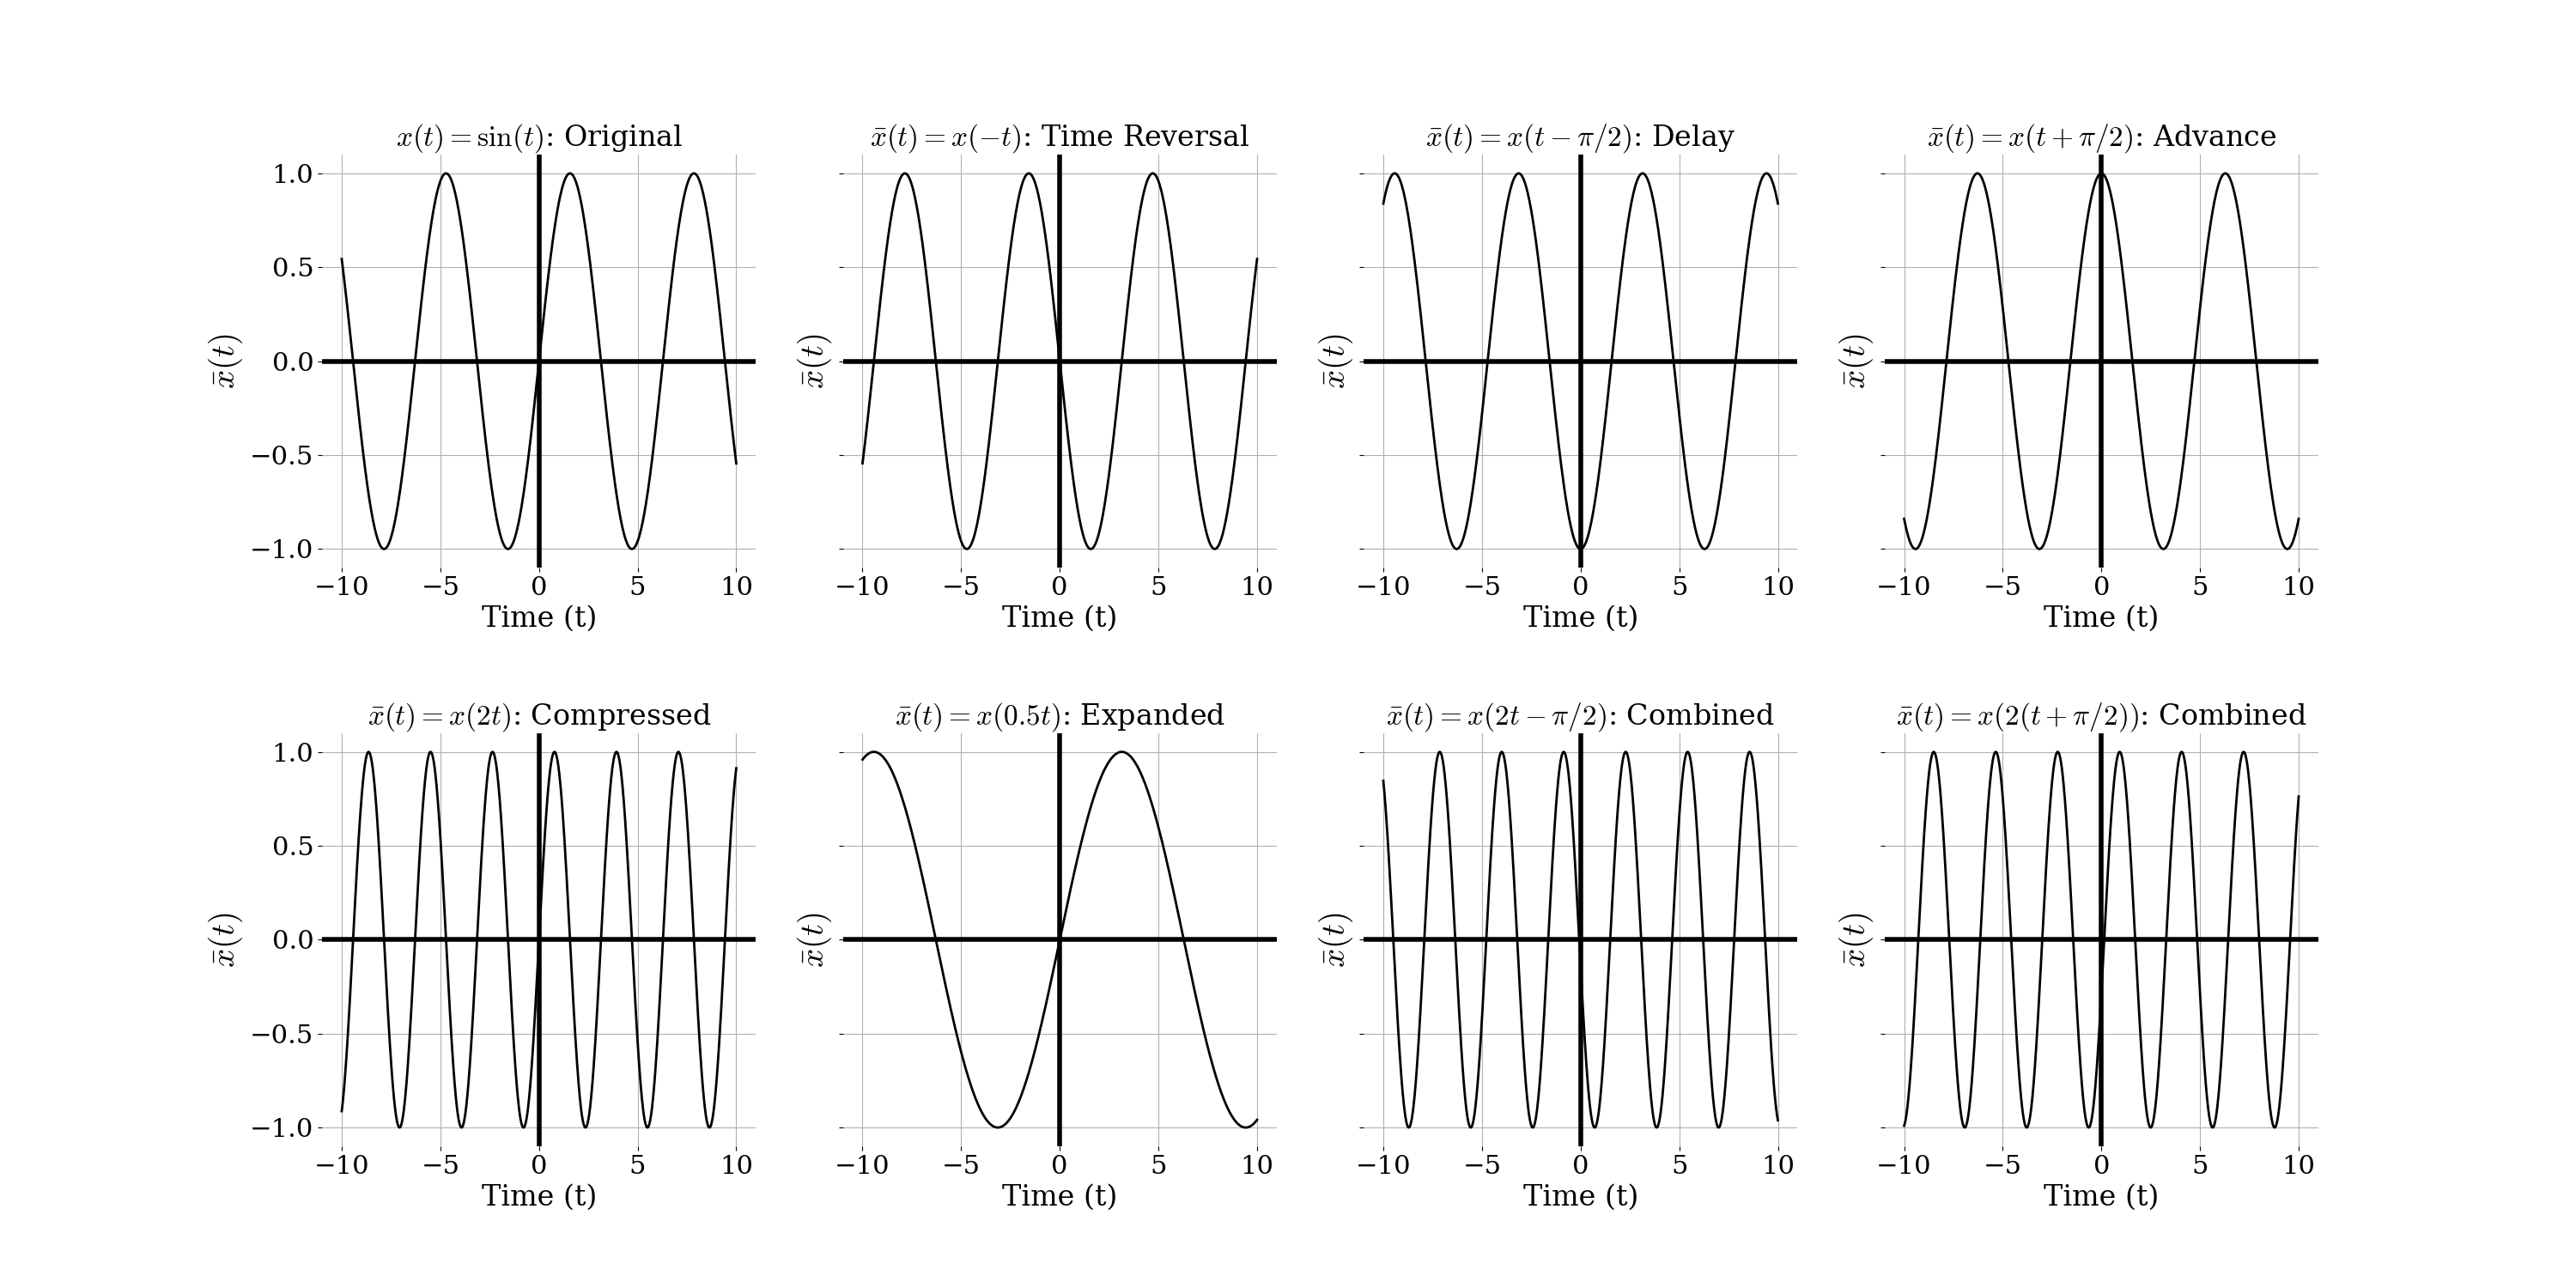
\includegraphics[width=\linewidth]{figs/signal_transformations.png}
    \caption{Time-shifting and time-scaling transformations of the signal $x(t) = \sin(t)$.}
    \label{fig:week2_sin}
\end{figure}
Note that for $\alpha = -1$, we get a reflection of the original signal across the vertical axis. Expanding on this example, we can also combine time-shifting and time-scaling operations to get more complex transformations. For instance, consider the transformation
\[
y(t) = x(\alpha t + t_0)
\]
where both $\alpha$ and $t_0$ are non-zero. This transformation first scales the time by $\alpha$ and then shifts it by $t_0$. The order of operations matters here --- if we were to shift first and then scale, we would have
\[
y(t) = x(\alpha (t + t_0)) = x(\alpha t + \alpha t_0)
\]
which is different from the previous transformation unless $\alpha = 1$.

If you intend to reverse the order of operations, you can redefine the shift parameter accordingly. For example, to achieve the same effect as $x(\alpha t + t_0)$ by shifting first and then scaling, you would need to use $x(\alpha (t + \frac{t_0}{\alpha}))$. Similarly, for the second combined transformation, you would need to use $x(\alpha t + \alpha t_0)$ to achieve the same effect as shifting first and then scaling by $\alpha$ next. Python code for generating signal transformations is available on Github\footnote{\href{https://github.com/ee-ucmerced/ee102-signals-systems/tree/main/lecture\_notes/week2/transformations.ipynb}{github.com/ee-ucmerced/ee102-signals-systems}}.

\subsection{Measuring the energy and power of signals}
Previously, we defined energy as the integral of the squared magnitude of a signal over all time:
\[E_\infty(x) = \int_{-\infty}^{\infty} |x(t)|^2 dt
\]
and power as the time-averaged measure for a time period $[-T, T]$:
\[
P_\infty(x) = \lim_{T \to \infty} \frac{1}{2T} \int_{-T}^{T} |x(t)|^2 dt.
\]

It is natural to wonder how we ended up with those specific definitions. You can build the intuition behind these definitions in two ways: (a) by considering an electrical signal $x(t)$ as a voltage across a 1-ohm resistor, and (b) by considering the mathematical convenience that these definitions provide. For (a), it is pretty clear that the energy dissipated in a resistor is given by the integral of the square of the voltage over time divided by the value of the resistor (in this case, 1 ohm). To fully appreciate the mathematical meaning of these definitions, consider the following alternate definition of energy as the integral of the absolute value of the signal over all time:
\[
E'_\infty(x) = \int_{-\infty}^{\infty} |x(t)| dt.
\]
This would be a valid way to quantify the ``energy'' of a signal as well. Note that our goal is to not physically define ``energy'', the electrical engineering concept, rather we are interested in coming up with measures of signals that we can use to compare two different signals. Note that taking absolute value is \textit{atleast} required to prevent the integral from being zero for signals that oscillate between positive and negative values. Despite this, the integral of the square of the absolute value ($E$) is preferred over just the integral of the absolute value ($E'$) because it is the metric that lets us compare signals in the $L^2$ space, which is a Hilbert space\footnote{Read more on Hilbert spaces here: \url{https://en.wikipedia.org/wiki/Hilbert_space}}. Simply stated, this means that the space of signals with finite energy (i.e., $E_\infty(x) < \infty$) has mathematical properties that enable better analysis and manipulation of signals. For example, we can define an inner product between two signals as a metric that quantifies the similarity between two signals $x(t)$ and $y(t)$ as \[
\langle x, y \rangle = \int_{-\infty}^{\infty} x(t) y^*(t) dt,
\]
where $y^*(t)$ is the complex conjugate of $y(t)$. This inner product allows us to define concepts like orthogonality and projection in the space of signals. \ul{Remember that} being able to represent complex signals as linear combinations of standard signals is the core concept in signal processing --- this is not possible without a clear notion of orthogonality! In fact, the definition of $E$ above is simply the inner product of a signal with itself, i.e., $E_\infty(x) = \langle x, x \rangle$. The $L^1$ space (signals with finite $E'$) does not have these properties, which is why we prefer to use $E$ as our measure of energy. Power can then be defined as the time-averaged energy over a time period.
\section{Periodic signals}
\begin{definition}
    A signal $x(t)$ is periodic if $\exists\,T_0>0$ such that $x(t+T_0)=x(t)$ for all $t$. The smallest such $T_0$ is the \emph{fundamental period} of the signal.
\end{definition}
In more verbose language, we say that a signal is a periodic signal if we can find a time shift $T_0$ such that shifting the signal by $T_0$ does not change the signal. If such a $T_0$ does not exist, then the signal is aperiodic. For example, $x(t)=\sin(t)$ is periodic. To find the fundamental period, we would have to find the smallest shift $T_0$ to satisfy $\sin(t+T_0)=\sin(t)$ for all $t$. Using the periodicity of the sine function, we know that $\sin(t+2\pi)=\sin(t)$ for all $t$. Thus, $T_0=2\pi$ is the fundamental period of $\sin(t)$. Note that $T_0=4\pi$ also satisfies the periodicity condition, but it is not the fundamental period since it is not the smallest such $T_0$. In fact, any integer multiple of $2\pi$ would satisfy the periodicity condition, but we are only interested in the smallest such value for the fundamental period. 

\subsection{Why periodic signals?} Just like many other concepts in signal processing, periodic signals are also a mathematical convenience! Intuitively, it is clear that if something repeats over and over again, then we can analyze just one cycle of it and extend the results to the entire signal. Therefore, studying periodic signals is often a good starting point. But you may wonder --- what if the signal is not periodic? Read on.

\subsection{Periodic extensions} 
When a signal is defined on a finite interval (e.g., a single cycle), it is often useful to \emph{periodically extend} it by repeating that interval end-to-end. This makes the time-averaged power well defined and makes symmetries/harmonics easier to see. 

\subsection{Example: Periodic or not?}
Consider the following three signals. Our goal is to find out whether they are periodic or not. If they are periodic, we will report the fundamental period of these signals.
\begin{enumerate}
    \item $x(t) = \cos(t)$
    \item $x(t) = \cos(t)$ for $ t \geq 0$ and $x(t) = -sin(t) $ for $t < 0$
    \item $x(t) = e^{j\omega t}$ where $\omega \neq 0$
\end{enumerate}

\textbf{How to prove periodicity?} We can simply \emph{propose a $T_0$ and check} if the periodicity condition is satisfied. If you cannot find a $T_0$, that does not mean that the signal is aperiodic --- it just means that you have not found the right $T_0$ yet! To prove aperiodicity, you have to show that no such $T_0$ exists. This is often done by contradiction. Proofs by contradiction is an important mathematical trick where you assume that the statement you want to prove is false and then show that this assumption leads to a contradiction (something that will be \emph{obviously} incorrect). This implies that the original statement must be true. You will find the signal transformation properties useful in proving (a)periodicity. Finally, if you can exploit the properties of the given signal, then you will find a much easier path to the proof.

For the first example, we know that the cosine function is ``oscillatory'', which indicates that it is probably periodic. Let's try to find a $T_0$ such that $\cos(t + T_0) = \cos(t)$ for all $t$. You might propose a $T_0 = \pi$ and observe that $\cos(t + \pi) = -\cos(t)$, which is not what we were looking for. So, $T_0 = \pi$ is not a good choice for $T_0$. Let's try one more time. Propose $T_0 = 2\pi$. Then, compute $\cos(t + 2\pi) = \cos(t)$, which is a valid choice. To check if it is the fundamental period, we can see that any integer multiple of $2\pi$ would also satisfy the periodicity condition, but $2\pi$ is the smallest such value. Therefore, the fundamental period of $x(t) = \cos(t)$ is $T_0 = 2\pi$. Note that you can use trignometric identities to help you prove periodicity in an alternate way too.

For the second signal, sketch the signal to first get an intuition about whether it is periodic or not. You will see that the signal is a cosine wave for $t \geq 0$ and a negative sine wave for $t < 0$. The two parts do not match at $t = 0$, which indicates that the signal is not periodic. To prove this, we can use contradiction. Assume that the signal is periodic with period $T_0$. Then, we have $\cos(t + T_0) = x(t + T_0) = x(t)$ for all $t$. Now, consider the case when $t = -\frac{T_0}{2}$. Then, we have $\cos(-\frac{T_0}{2} + T_0) = \cos(\frac{T_0}{2}) = x(-\frac{T_0}{2}) = -\sin(-\frac{T_0}{2}) = \sin(\frac{T_0}{2})$. This is clearly not true! So, our assumption that the signal is periodic must be false. Therefore, the signal is aperiodic.

For the third signal, we can use the properties of the complex exponential function to prove periodicity. Write $x(t + T_0) = e^{j\omega(t + T_0)} = e^{j\omega t}e^{j\omega T_0}$. If we can find a $T_0$ such that $e^{j\omega T_0} = 1$, then we have periodicity. This is satisfied if $T_0 = \frac{2\pi}{\omega}$. Therefore, the fundamental period of $x(t) = e^{j\omega t}$ is $T_0 = \frac{2\pi}{\omega}$.

% Memoryless nonlinearities (like clipping) do not change $T_0$ but \emph{do} add harmonics (distortion) while preserving periodicity.

\subsection{Power and energy of periodic signals}
We can revisit the power and energy definitions for periodic signals. If $x$ is periodic with period $T_0$, then the time-average power is well defined and can be computed over any interval of length $T_0$. Note that for a finite-duration input, $E_\infty$ is finite and $P_\infty=0$ (time average over an unbounded window goes to zero) whereas $E_\infty$ is finite because we have finite-duration signal. For periodic signals, we have
\[
P_\infty(x)=\frac{1}{T_0}\!\int_{t_0}^{t_0+T_0}\!|x(t)|^2 dt
\quad(\text{independent of }t_0),\qquad
E_\infty(x)=\infty\ \text{unless }x\equiv 0.
\]
Thus, periodic signals are \emph{power signals} (finite power, infinite energy).
\subsection*{Energy and power for a periodic input}
If $x(t)$ is periodic with fundamental period $T_0$, then $y_d(t)$ is also periodic with the \emph{same} $T_0$ (memoryless mapping preserves period). Hence
\[
E_\infty(y_d)=\int_{-\infty}^{\infty}\!|y_d(t)|^2\,dt=\infty,\qquad
P_\infty(y_d)=\frac{1}{T_0}\int_{t_0}^{t_0+T_0}\!|y_d(t)|^2\,dt\ \text{(finite)}.
\]

\section{Even and odd signals}
Recall that a mathematical function is called even if $f(-t)=f(t)$ for all $t$ and odd if $f(-t)=-f(t)$ for all $t$. Examples of even functions include $\cos(t)$, $t^2$, and $|t|$. Examples of odd functions include $\sin(t)$, $t^3$, and the sign function $\text{sgn}(t)$.
\begin{definition} A signal $x(t)$ is even if $x(-t)=x(t)$ for all $t$ and odd if $x(-t)=-x(t)$ for all $t$.
\end{definition}

\begin{proposition}
    Any signal $x(t)$ can be uniquely decomposed as the sum of an even signal $x_e(t)$ and an odd signal $x_o(t)$.
\end{proposition}
\begin{proof}
    Let $x_e(t)=\frac{x(t)+x(-t)}{2}$ and $x_o(t)=\frac{x(t)-x(-t)}{2}$. Then, we have
    \[
    x_e(-t) = \frac{x(-t) + x(t)}{2} = x_e(t)
    \]
    so $x_e(t)$ is even. Similarly,
    \[
    x_o(-t) = \frac{x(-t) - x(t)}{2} = -x_o(t).
    \]
    which is is odd. Now, we can see that
    \[
    x_e(t) + x_o(t) = \frac{x(t) + x(-t)}{2} + \frac{x(t) - x(-t)}{2} = x(t).
    \]
    To prove uniqueness, we again use the proof by contradiction method. Assume, to the contrary, that there exist another pair of even and odd signals $x'_e(t)$ and $x'_o(t)$ such that $x(t) = x'_e(t) + x'_o(t)$. Then, we have
    \[
    x_e(t) - x'_e(t) = x'_o(t) - x_o(t).
    \]
    The left side is even (difference of two even functions), and the right side is odd (difference of two odd functions). The only function that is both even and odd is the zero function. Therefore, we have $x_e(t) - x'_e(t) = 0$ and $x'_o(t) - x_o(t) = 0$, which implies that $x_e(t) = x'_e(t)$ and $x_o(t) = x'_o(t)$. Hence, the decomposition is unique.
\end{proof}

\section{Application demonstration: a guitar amplifier}
An amplifier system can be modeled as $y(t) = \alpha x(t)$ where $\alpha > 1$ is the amplifier gain. However, real-world amplifiers have limits on the maximum and minimum output levels they can produce. When the input signal is too large, the output signal gets ``clipped'' at these limits. Although this is an undesirable effect for most audio applications, it is often used intentionally by musicians to create a distorted sound effect. This is common in many music genres such as rock, metal, and punk. 

We can model a simple hard-clipping (overdrive) amplifier system as:
\[
y_d(t)=
\begin{cases}
-\beta, & \alpha\,x(t)<-\beta,\\[2pt]
\alpha\,x(t), & |\alpha\,x(t)|\le \beta,\\[2pt]
\beta, & \alpha\,x(t)>\beta,
\end{cases}
\qquad \alpha>0,\ \beta>0.
\]
This is a \emph{memoryless} nonlinearity: at each $t$, $y_d(t)$ depends only on $x(t)$. It amplifies small inputs by $\alpha$ and saturates at $\pm\beta$ for large inputs.
Here, the parameter $\alpha$ controls the amount of gain (loudness) and $\beta$ controls the amount of distortion to apply. Vierinen has a YouTube demonstration for this effect\footnote{\url{https://youtu.be/I30Mn_-yYF8.}}.

The transfer curve for this system is shown in Figure~\ref{fig:sys_clip}. 
% \subsection*{Transfer curve (draw in class)}
\begin{figure}[h]
\centering
\begin{tikzpicture}[>=latex,scale=1.0]
  % axes
  \draw[->] (-4.2,0)--(4.6,0) node[below] {$\alpha\,x$};
  \draw[->] (0,-2.8)--(0,2.8) node[left] {$y_d$};

  % clip levels
  \draw[dashed,gray] (-4,2) -- (4,2) node[right] {$\beta$};
  \draw[dashed,gray] (-4,-2) -- (4,-2) node[right] {$-\beta$};

  % linear segment
  \draw[line width=1.2pt] (-2,-2) -- (2,2); % slope 1 in αx–yd plane

  % saturated segments
  \draw[line width=1.2pt] (-4,-2) -- (-2,-2);
  \draw[line width=1.2pt] (2,2) -- (4,2);

  % ticks
  \draw (2,0.08)--(2,-0.08) node[below=2pt] {$\beta$};
  \draw (-2,0.08)--(-2,-0.08) node[below=2pt] {$-\beta$};
\end{tikzpicture}
\caption{Hard-clipping nonlinearity: linear region $|\alpha x|\le \beta$, saturation outside.}
\label{fig:sys_clip}
\end{figure}

\textbf{Transforming the system:} You can apply all the signal transformations to transform the system by transforming the transfer curve of the system shown above. Using Python, try to draw all time operations discussed above for $y_d(t)$ --- the distorting amplifier system. Figure~\ref{fig:week2_clipping} shows the results.
\begin{figure}
    \centering
    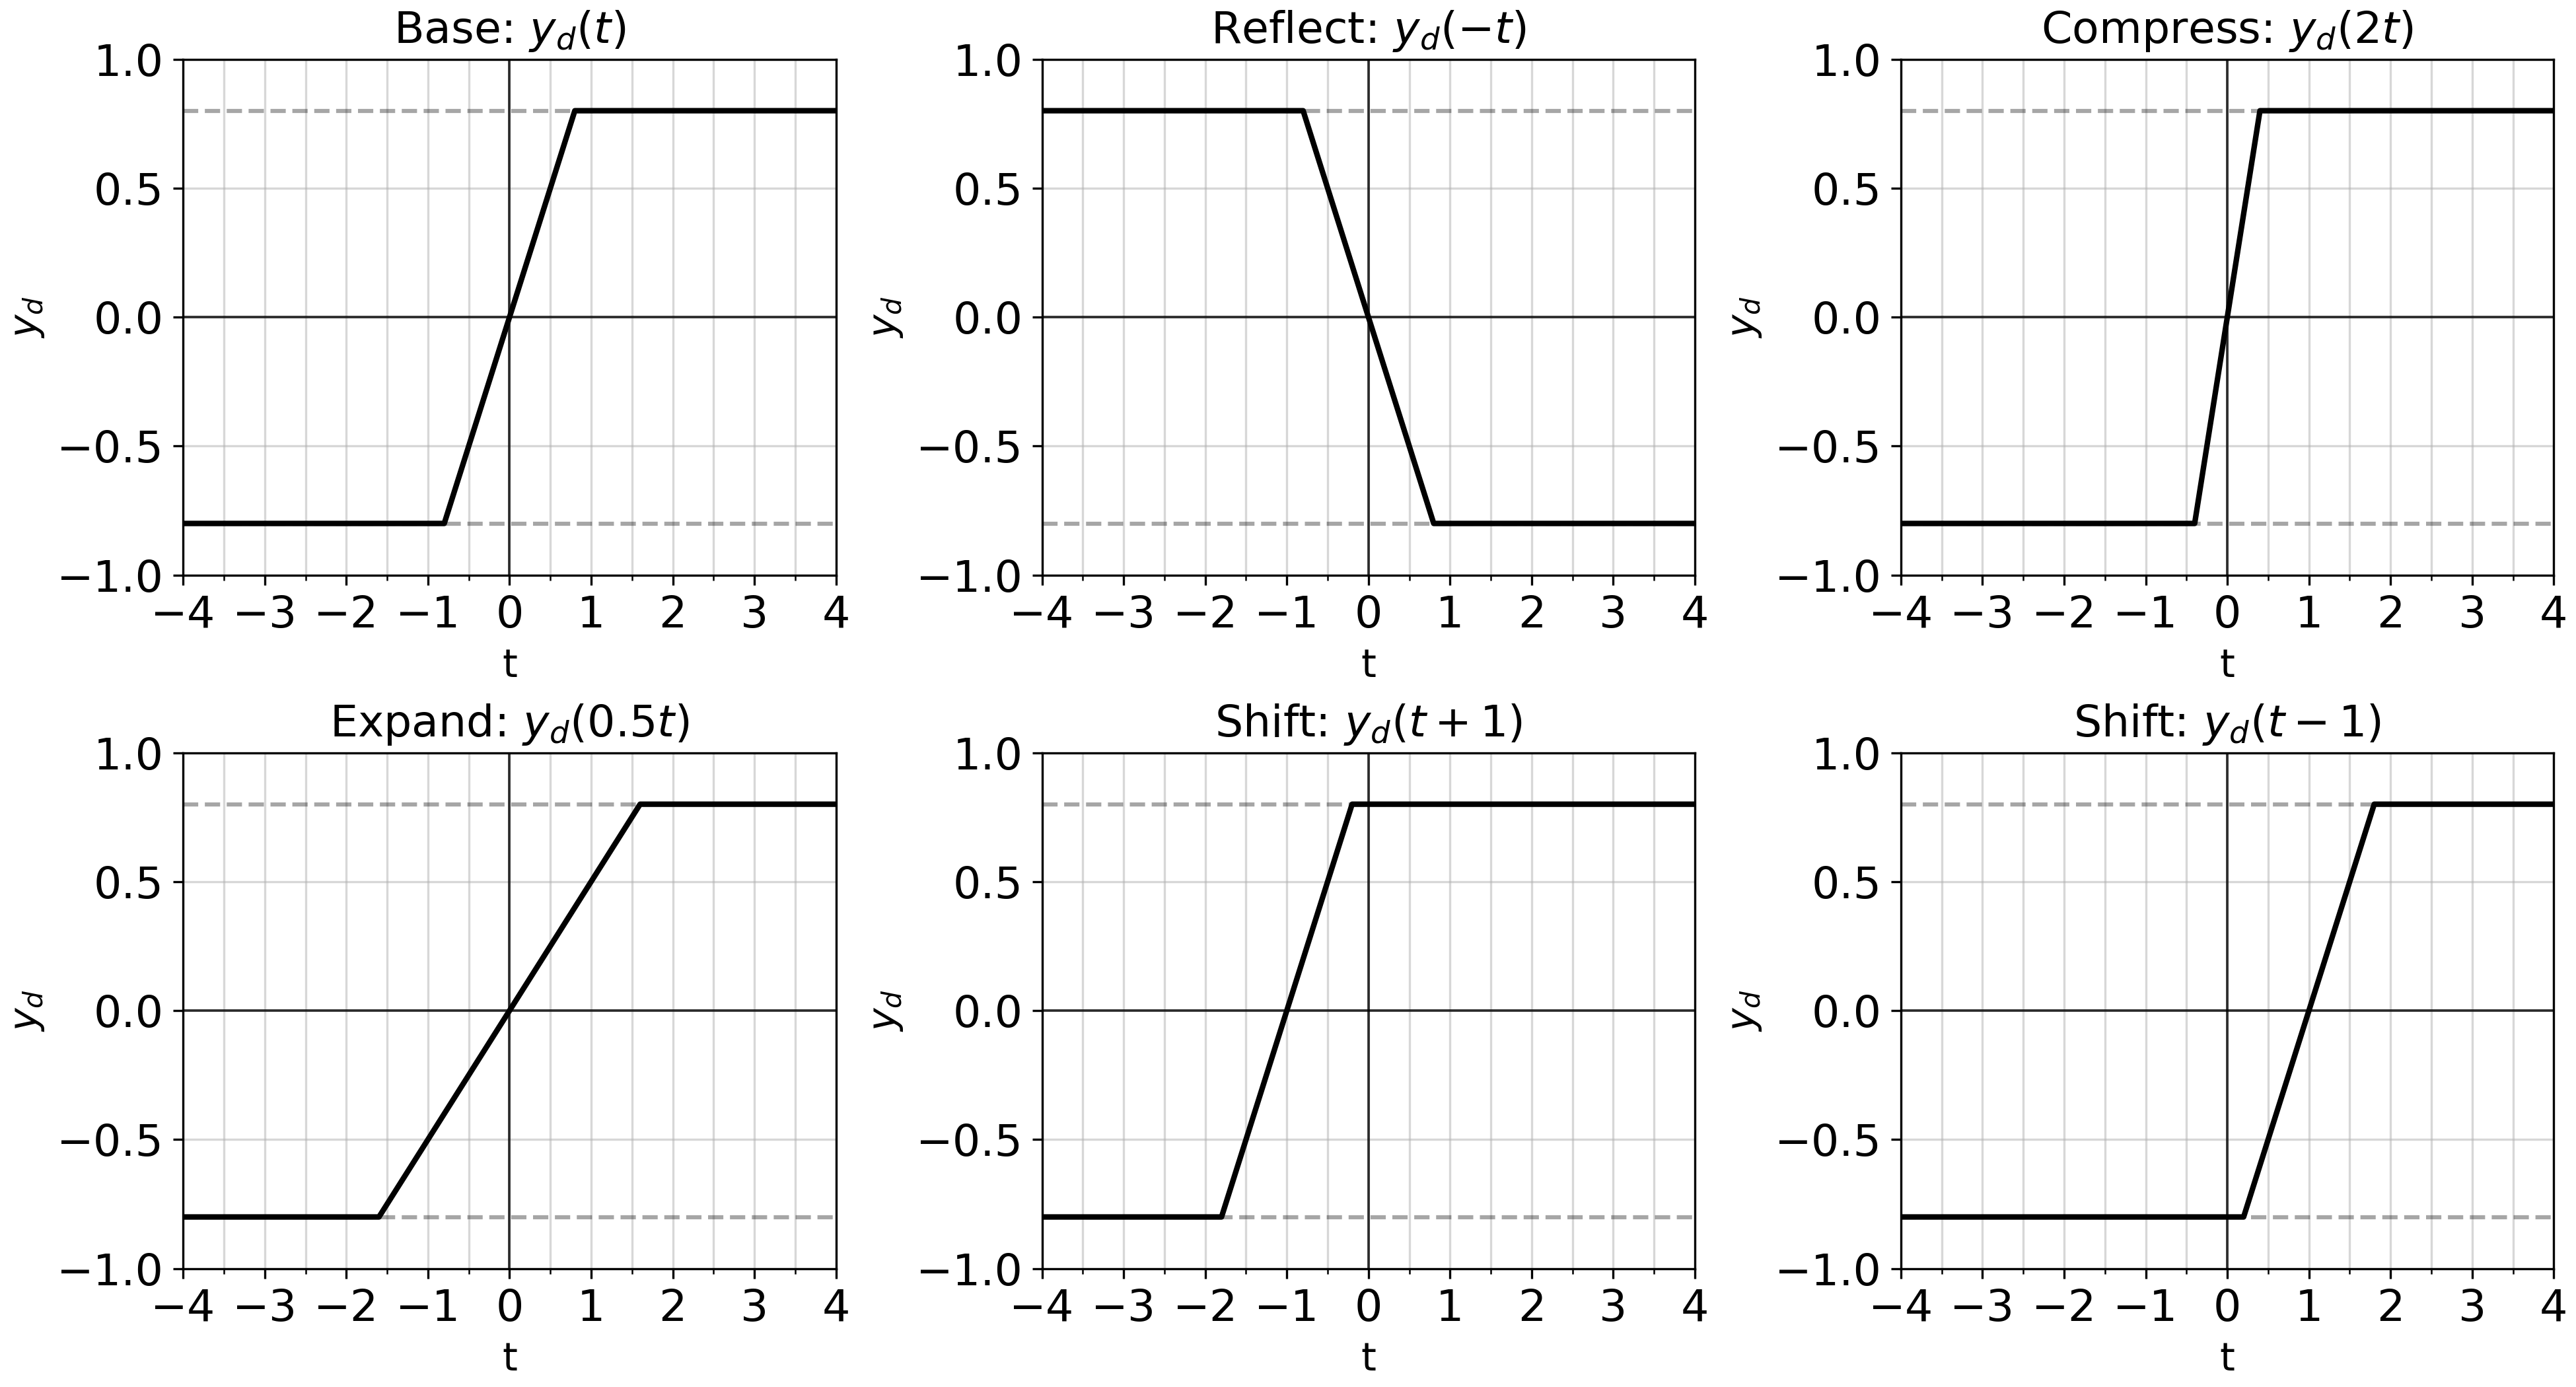
\includegraphics[width=\linewidth]{figs/clip_ops_grid.png}
    \caption{Time operations on the signal $y_d(t)$.}
    \label{fig:week2_clipping}
\end{figure}

\subsection{Distortion effects}
By running the provided code, you can test various distortion effects by changing the parameters $\alpha$ and $\beta$. The code loads a .wav file for a sample guitar tone. Practice your Python (and music design) skills with this example!
\subsection{Optional: Audio tone signal example and time operations}
In the supplementary notes, you will find a Python notebook that creates a guitar-like audio tone. You can use computer programming to compute various time-transformed versions yourself.

\section*{Next class}
The unit impulse $\delta(t)$ and step $u(t)$; convolution preview.

\end{document}
